The training of recurrent neural networks is afflicted by the so called \textit{exploding} and \textit{vanishing} gradient problem; such problem is directly linked to
the notion of memory. When we talk about memory what are we really talking about is the dependecy of neuron output at a given time $t$ from previous time steps,
that is how $\phi^t$ depends on $\phi^{k}$ with $t>k$. This dependecy is captured by the expression $\frac{\partial \vec{a}^t}{\partial \vec{a}^k}$.
Obiuvsly when such expression equals zero it means neuron output at time $t$ is not affected by output at time $k$, so if this situation occurs during training
we have no hope to produce output sequence that take into consideration input sequence components previous  to time $k$.
The terms $\frac{\partial \vec{a}^t}{\partial \vec{a}^k}$ are usually referred as \textit{long term} contribution when $k<<t$ or \textit{short term} contributions
otherwise.

We talk of \textit{exploding} gradient problem when \textit{long term} components grow exponentially, on the contrary of \textit{short term} ones, causing
the overall norm of the gradient to explode.
We refer to \textit{vanishing} gradient problem when, vice versa, \textit{long terms} diminish exponentially.


We have seen in the previous section that
\begin{equation}
\frac{\partial \vec{a}^t}{\partial \vec{a}^k} = \prod_{i=t-1}^{k}  diag(\sigma'(\vec{a}^i)) \cdot \mat{W}^{rec}
\label{memory_eq}
\end{equation}
Intuitively we can understand why such problems arises, more evidently in \textit{long term} components, just by looking at equation \ref{memory_eq};
We can notice each temporal contribution is the product of $l=t-k-1$ jacobian matrix, so in \textit{long term} components $l$ is large and depening on
eigenvalues of the matrixes in the product we can go exponentially fast towards 0 or infinty.

Let's now dig a bit deeper and rewrite equation \ref{memory_eq} with respect to a couple of neurons $i$ and $j$

\begin{equation} 
\frac{\partial \vec{a}_i^t}{\partial \vec{a}_j^k} = \sum_{q\in P(j)} \sum_{l \in P(q)} \hdots \sum_{h : i \in P(h)} w_{qj} \hdots w_{jh} \cdot \sigma'(a_j^k)\sigma'(a_q^{k+1}) \hdots \sigma'(a_i^{t-1})
\label{expanded_mem}
\end{equation}


Observing the previous equation we can argue that each derivatives it's the sum of $p^{t-k-1}$ terms; each term represents the path cost from neuron $i$ to neuron $j$ in the unfolded network, obviously
there are $p^{t-k-1}$ such paths. If we bind the cost $\sigma'(a_l^t)$ to neuron $l$ in the $t^{th}$ layer in the unfolded network we can read the path cost simply surfing the unfolded network multiply
the weight of each arc we walk through and the cost of each neuron we cross, as we can see from figure \ref{gradient_path_cost}.


\tikzstyle{rnn_style}=[->,shorten >=1pt,auto,node distance=1.5cm,
  thick,
  neuron/.style={circle,fill=white!50,draw,minimum size=0.7cm,inner sep=0pt,font=\sffamily\normalsize},
  missing/.style={circle,fill=white!50,draw=none,minimum size=0.7cm,font=\sffamily\Huge\bfseries},
  label/.style={node distance=1.2cm,rectangle,fill=white!50,draw=none,minimum size=0.7cm,font=\sffamily\normalsize},
  thick_edge/.style={line width=1.2pt},
  thin_edge/.style={dotted, line width=0.5pt},
  weight/.style = {above,sloped,pos=0.3},
  ]
\begin{figure}
 \centering
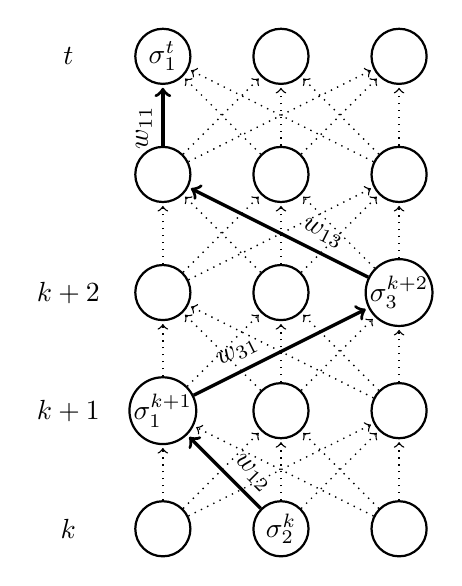
\begin{tikzpicture}[rnn_style]

  
  \node[neuron]    (x1)[]   {$\sigma_1^t$};
  \node[neuron]    (x2)[right of=x1]   {};
  \node[neuron]    (x3)[right of=x2]   {};
  \node[label]     (xl)[left of=x1] {$t$};
  
  \node[neuron]    (h1)[below of =x1]   {$\hdots$};
  \node[neuron]    (h2)[right of=h1]   {};
  \node[neuron]    (h3)[right of=h2]   {};
  \node[label]     (hl)[left of=h1] {$\hdots$};
  
  \node[neuron]    (y1)[below of=h1]   {};
  \node[neuron]    (y2)[right of=y1]   {};
  \node[neuron]    (y3)[right of=y2]   {$\sigma_3^{k+2}$};
  \node[label]     (yl)[left of=y1] {$k+2$};

  
  \node[neuron]    (z1)[below of=y1]   {$\sigma_1^{k+1}$};
  \node[neuron]    (z2)[right of=z1]   {};
  \node[neuron]    (z3)[right of=z2]   {};
  \node[label]     (zl)[left of=z1] {$k+1$};
  
  \node[neuron]    (w1)[below of=z1]   {};
  \node[neuron]    (w2)[right of=w1]   {$\sigma_2^k$};
  \node[neuron]    (w3)[right of=w2]   {};
  \node[label]     (wl)[left of=w1] {$k$};

  
%   \node[label]      (lu)[left of=u] {$u$};
%   \node[label]      (ll)[left of=z1] {$l$};


  \path[->] (h1) edge [thick_edge] node[weight]{$w_{11}$}  (x1)
	    (h1) edge [thin_edge]   (x2)
	    (h1) edge [thin_edge]   (x3)
	    (h2) edge [thin_edge]  (x1)
	    (h2) edge [thin_edge]   (x2)
	    (h2) edge [thin_edge]   (x3)
	    (h3) edge [thin_edge]  (x1)
	    (h3) edge [thin_edge]   (x2)
	    (h3) edge [thin_edge]   (x3);

  \path[->] (y1) edge [thin_edge]   (h1)
	    (y1) edge [thin_edge]   (h2)
	    (y1) edge [thin_edge]   (h3)
	    (y2) edge [thin_edge]   (h1)
	    (y2) edge [thin_edge]   (h2)
	    (y2) edge [thin_edge]   (h3)
	    (y3) edge [thick_edge] node[weight]{$w_{13}$}   (h1)
	    (y3) edge [thin_edge]   (h2)
	    (y3) edge [thin_edge]   (h3);
  
  
  \path[->] (z1) edge [thin_edge]   (y1)
	    (z1) edge [thin_edge]  (y2)
	    (z1) edge [thick_edge] node[weight]{$w_{31}$}   (y3)
	    (z2) edge [thin_edge]  (y1)
	    (z2) edge [thin_edge]  (y2)
	    (z2) edge [thin_edge]  (y3)
	    (z3) edge [thin_edge]   (y1)
	    (z3) edge [thin_edge]   (y2)
	    (z3) edge [thin_edge]   (y3);
	    
  \path[->] (w1) edge [thin_edge]   (z1)
	    (w1) edge [thin_edge]  (z2)
	    (w1) edge [thin_edge]   (z3)
	    (w2) edge [thick_edge] node[weight]{$w_{12}$}   (z1)
	    (w2) edge [thin_edge]   (z2)
	    (w2) edge [thin_edge]   (z3)
	    (w3) edge [thin_edge]   (z1)
	    (w3) edge [thin_edge]   (z2)
	    (w3) edge [thin_edge]   (z3);

	    


\end{tikzpicture}
\caption{The cost for a path from neuron $2$ at time $k$ to neuron $1$ at time $t$ is $w_{12}w_{31}w_{13}\hdots w_{11}\cdot \sigma_2^k \sigma_1^{k+1}\sigma_3^{k+2} \hdots \sigma_1^{t-1} $ }
\label{gradient_path_cost}
\end{figure}


We can further characterize each path cost noticing that we can separate two components, one that depends only on the weights $w_{qj} \hdots w_{jh}$ and the other that depends both on the weights and the inputs
$\sigma'(a_j^k)\sigma'(a_q^{k}) \hdots \sigma'(a_i^{t-1})$.


\paragraph{Hochreiter Analysis: Weak upper bound}
In this paragraph we report some useful consideration made by Hochreiter, please see \cite{Hochreiter95longshort-term} for more details.

Let's put $$\sigma'_{max} \triangleq \underset{i=k,...,t-1}{\text{max  }} \{||diag(\sigma'(a^i))||_1\}$$.

We have then:
$$\left\Vert \prod_{i=t-1}^{k}  diag(\sigma'(\vec{a}^i)) \cdot \mat{W}^{rec} \right\Vert_1 <= \prod_{i=t-1}^{k} p \cdot ||diag(\sigma'(\vec{a}^i))||_1 \cdot ||\mat{W}^{rec}||_1 $$
since 
$$||diag(\sigma)\cdot \mat{W}||_1 =
\left\Vert 
\begin{array}{c c c c}
\sigma_1 w_{11} & \sigma_1 w_{12} & \hdots & \sigma_1 w_{1p}  \\
\sigma_1 w_{21} & \sigma_2 w_{22} & \hdots & \sigma_2 w_{2p}  \\
\vdots & \vdots  & \vdots & \vdots  \\
\sigma_p w_{p1} & \sigma_p w_{p2} & \hdots & \sigma_p w_{pp}  \\
\end{array}  
\right\Vert_1
<=p \cdot \sigma_{max} \cdot ||\mat{W}||_1
$$

Hence
\begin{align}
\left\Vert \prod_{i=t-1}^{k}  diag(\sigma'(\vec{a}^i)) \cdot \mat{W}^{rec} \right\Vert_1 & <= p \cdot \big(\sigma'_{max}\cdot ||\mat{W}||_1\big)^{t-k-1} \\
& = p \cdot \tau^{t-k-1}
\end{align}
where $$\tau \triangleq \sigma'_{max}\cdot ||\mat{W}||_1$$

So we have exponential decay if $\tau<1$; We can match this condition if
$$\frac{p\cdot ||w_{max}||}{\sigma_{max}}<1$$ where $w_{max}$ is the maxixum value in the weight matrix.

As pointed out by Hochreiter in his work we can match this condition, in the case of sigmoid activation function by choosing $w_{max} < \frac{4}{n}$.

\paragraph{The ReLU case}

Relu case is a bit special, because of it's derivative.
\begin{align}
  \sigma(x)&=\begin{cases}
    x & \text{if $x>0$}.\\
    0 & \text{otherwise}.
  \end{cases} \\ 
    \sigma'(x)&=\begin{cases}
    1 & \text{if $x>0$}.\\
    0 & \text{otherwise}.
  \end{cases}
\end{align}
Relu's derivative is a step function, it can assume only two values: $1$ when the neuron is active, $0$ otherwise.
Returning to the path graph we introduced earlier we can say that a path is \textit{enabled} if each neuron in that path is active. In fact if we
encounter a path wich cross a non active neuron it's path cost will be 0; on the contrary for an \textit{enabled} path thw cost will be simply the product
of weight of the arcs we went through, as we can see in figure \ref{gradient_path_cost_relu}


\tikzstyle{rnn_style}=[->,shorten >=1pt,auto,node distance=1.5cm,
  thick,
  neuron/.style={circle,fill=white!50,draw,minimum size=0.7cm,inner sep=0pt,font=\sffamily\normalsize},
  missing/.style={circle,fill=white!50,draw=none,minimum size=0.7cm,font=\sffamily\Huge\bfseries},
  label/.style={node distance=1.2cm,rectangle,fill=white!50,draw=none,minimum size=0.7cm,font=\sffamily\normalsize},
  thick_edge/.style={line width=1.2pt},
  thin_edge/.style={dotted, line width=0.5pt},
  weight/.style = {above,sloped,pos=0.3},
  blacked/.style={fill=black},
  ]
\begin{figure}
 \centering
\begin{tikzpicture}[rnn_style]

  
  \node[neuron,blacked]    (x1)[]   {};
  \node[neuron]    (x2)[right of=x1]   {};
  \node[neuron]    (x3)[right of=x2]   {};
  \node[label]     (xl)[left of=x1] {$t$};
  
  \node[neuron,blacked]    (h1)[below of =x1]   {};
  \node[neuron]    (h2)[right of=h1]   {};
  \node[neuron]    (h3)[right of=h2]   {};
  \node[label]     (hl)[left of=h1] {$\hdots$};
  
  \node[neuron]    (y1)[below of=h1]   {};
  \node[neuron]    (y2)[right of=y1]   {};
  \node[neuron,blacked]    (y3)[right of=y2]   {};
  \node[label]     (yl)[left of=y1] {$k+2$};

  
  \node[neuron,blacked]    (z1)[below of=y1]   {};
  \node[neuron]    (z2)[right of=z1]   {};
  \node[neuron]    (z3)[right of=z2]   {};
  \node[label]     (zl)[left of=z1] {$k+1$};
  
  \node[neuron]    (w1)[below of=z1]   {};
  \node[neuron,blacked]    (w2)[right of=w1]   {};
  \node[neuron]    (w3)[right of=w2]   {};
  \node[label]     (wl)[left of=w1] {$k$};

  
%   \node[label]      (lu)[left of=u] {$u$};
%   \node[label]      (ll)[left of=z1] {$l$};


  \path[->] (h1) edge [thick_edge] node[weight]{$w_{11}$}  (x1)
	    (h1) edge [thin_edge]   (x2)
	    (h1) edge [thin_edge]   (x3)
	    (h2) edge [thin_edge]  (x1)
	    (h2) edge [thin_edge]   (x2)
	    (h2) edge [thin_edge]   (x3)
	    (h3) edge [thin_edge]  (x1)
	    (h3) edge [thin_edge]   (x2)
	    (h3) edge [thin_edge]   (x3);

  \path[->] (y1) edge [thin_edge]   (h1)
	    (y1) edge [thin_edge]   (h2)
	    (y1) edge [thin_edge]   (h3)
	    (y2) edge [thin_edge]   (h1)
	    (y2) edge [thin_edge]   (h2)
	    (y2) edge [thin_edge]   (h3)
	    (y3) edge [thick_edge] node[weight]{$w_{13}$}   (h1)
	    (y3) edge [thin_edge]   (h2)
	    (y3) edge [thin_edge]   (h3);
  
  
  \path[->] (z1) edge [thin_edge]   (y1)
	    (z1) edge [thin_edge]  (y2)
	    (z1) edge [thick_edge] node[weight]{$w_{31}$}   (y3)
	    (z2) edge [thin_edge]  (y1)
	    (z2) edge [thin_edge]  (y2)
	    (z2) edge [thin_edge]  (y3)
	    (z3) edge [thin_edge]   (y1)
	    (z3) edge [thin_edge]   (y2)
	    (z3) edge [thin_edge]   (y3);
	    
  \path[->] (w1) edge [thin_edge]   (z1)
	    (w1) edge [thin_edge]  (z2)
	    (w1) edge [thin_edge]   (z3)
	    (w2) edge [thick_edge] node[weight]{$w_{12}$}   (z1)
	    (w2) edge [thin_edge]   (z2)
	    (w2) edge [thin_edge]   (z3)
	    (w3) edge [thin_edge]   (z1)
	    (w3) edge [thin_edge]   (z2)
	    (w3) edge [thin_edge]   (z3);

	    


\end{tikzpicture}
\caption{The cost for an enabled path from neuron $2$ at time $k$ to neuron $1$ at time $t$ is $w_{12}w_{31}w_{13}\hdots w_{11}$ }
\label{gradient_path_cost_relu}
\end{figure}


So $\vert (\frac{\partial \vec{a}^t}{\partial \vec{a}^k})_{ij}\vert$ ranges from 0, when no path is enabled to, $\vert ((\mat{W}^{rec})^{t-k-1})_{ij} \vert$ when all
paths are enabled, which is a more strict bound that what we can find with Hochreiter analysis.



COMPORTAMENTO SBALIATO STRUTTURALE\\
RELU-NON POSSIAMO IMPARARE AD ACCENDERE \\





